
\subsection{Skyline Query}\label{sec:skyline_operator}

Skyline query is an operation that finds all data records which
are not dominated by any other data objects in a given data set.
Skyline query is closely related to the maximal vector
problem~\cite{Kung75onfinding,conf/vldb/GodfreySG05}. Here, we
briefly introduce these concepts.

%define the terms that are used to formally define maximal vectors
%and skyline operator. The concept of \emph{attribute domains},
%though intuitive, is also defined here and will be used to
%formally define \emph{pruning region}, which is the core idea used
%in the solution section of this paper.

%We use $n$ to denote the number of dimension of the skyline query,
%and only consider attributes in the data set that are interested
%for skyline query. Non-skyline attributes are only used for
%clarification of illustrations.

%\begin{definition}[Record] Given the set of domains of totally
%ordering sets $D$ = \{$D_1$, $D_2$, ... $D_n$\} and a set of
%attributes $A$ = \{$A_1$, $A_2$, ... $A_n$\}, a records, denoted
%by $p$, is a n-tuple $p$ = ($A_1$, $A_2$, ... $A_n$) such that
%$A_i$ $\epsilon$ $D_i$ for $i$ = 1 to $n$.
%\end{definition}

%\begin{definition}[Data Set]
%Data set, denoted by $P$ is a set of data records denoted by $P$ =
%\{$p_1$, $p_2$, ..., $p_m$\}, where $m$ is the number of tuples in
%the data set.
%\end{definition}

%Figure~\ref{tab:sample_data} shows an example of a data set where
%the domain of the first attribute is alphabets; the domain for the
%second and the third attribute is the set of positive real
%numbers, $\mathbb{R}^+$.

%The skyline operation has been known as the problem of
%finding maximal vectors from a set of vectors as
%studied in \cite{Kung75onfinding}. Maximal vectors are defined as  follows:

\begin{definition}[Maximal Vector]\label{def:max_vector}
Given the set of vectors $P$, for all vectors $v$ $\epsilon$ $P$,
there does not exist $u$ $\epsilon$ $P$ such that $u$ $\geq$ $v$,
then $v$ is a maximal vector.

\begin{equation}\label{eq:max_vector}
    MaxVect(P) = \{v | \forall v, u \epsilon P \nexists u \geq v\}
\end{equation}

\end{definition}

The comparison operator $\geq$ used in
Equation~\ref{eq:max_vector} is defined on vectors such that for
two vectors $u$, $v$ $\epsilon$ $V$, $u$ $\geq$ $v$ if $u_i$
$\geq$ $v_i$ for $i$ = 1 to $n$. Vice versa for the $\leq$
operator. In other words, a vector $v$ is ``greater than" the
other vector $u$ if and only if all elements of $v$ is ``greater
than or equal to'' all elements of $u$. The comparison operators
for each element of the vectors are the natural ordering operators
defined on each domain.

The only difference between the maximal vector operation defined
in definition \ref{def:max_vector} and the skyline operation is
that the skyline operator defines a set of \emph{preference
specifiers}, $\sigma$, which are to be either \emph{MIN} or
\emph{MAX} for each attribute.

%In addition, the skyline operator defines the preference specifier for
%each relevant skyline attribute. The preference specifiers, $\sigma$,
%is a set of Minimize (MIN) or Maximize (MAX) specifiers that defines
%the dominance relationship on each attribute. For a attribute with a
%MIN specifier, a lower value from the domain of the attribute dominates
%a higher value.

%The $\geq$ operator is defined based on the ordering
%of the domain. We redefined the $\geq$ operator to be the
%dominance relationship. In this case, skyline can be defined
%using the finding maximal vector problem.

\begin{definition}[Skyline Operator]\label{def:skyline}
Give a set of tuples, $P$, and an ordered set of preference
specifiers, $\sigma$, the skyline operator is defined as follows:

\begin{equation}\label{eq:skyline}
    Skyline(P, \sigma) = MaxVect(P)
\end{equation}

\end{definition}

In definition~\ref{def:skyline}, the dominance relationship is
defined as follows:

\begin{definition}[Dominance Relationship]\label{def:dom_rel}
Give two points $p_1$ and $p_2$ in $P$, $p_1$ dominates $p_2$, if
and only if all elements of $p_1$ dominates or is equal to all
elements of $p_2$ and at least one element is dominant. Dominance
for each element depends on the preference specifier, $\sigma_i$,
for that attribute. Given $x$ and $y$ from $D_i$, the domanance
for the elements is defined as follows:

\begin{enumerate}
\item If $\sigma_i$ = \emph{MIN}, $x$ {\bf dominates} $y$ if $x$
$<$ $y$. \item If $\sigma_i$ = \emph{MAX}, $x$ {\bf dominates} $y$
if $x$ $>$ $y$.
\end{enumerate}

\end{definition}

\begin{corollary}\label{co:dom_rel}
The dominance relationship is transitive, non-reflexive, and
non-symmetric.
\end{corollary}

\begin{proof}
All three properties can be proven based on the fact that the values of
each attribute domain are ordered: an attribute $x$ is better than $y$ then,
$y$ is worse than $x$. The transitive property of the dominance relationship
follows
from Definition~\ref{def:dom_rel}, if record $A$ dominates $B$ then all
attributes of $A$ are equal or better and there is at least one attribute
that is better; therefore, $B$ dominates $C$ implies that all attributes
of $A$ is
equal or better than $C$ therefore, the relationship is transitive.
The relationship is non-reflexive since if all attribute of $A$ is equal
or better than attribute of $B$ then the ordering of the values of each
attribute domain imply that $B$ does not dominate
$A$. Similarly, $D$ does not dominate itself since the definition states
that at least one must be better for a record to dominate another.
\end{proof}

Following the non-reflexive property of Corollary~\ref{co:dom_rel}, given
two record $A$ and $B$ and $A = B$, if $A$ is a skyline record, then
$B$ is also a skyline record.

Extension SQL syntax for skyline was defined by B\"{o}rzs\"{o}nyi,
et al. in \cite{skyline_operator} as illustrated in Figure
\ref{fig:skyline_sql}. The syntax defines an additional SKYLINE
clause in SQL that specifies how the skyline operation should be
performed. In the SKYLINE clause, relevant attributes (such as
H.price and H.dist in the figure) can be listed. For each
attribute, the syntax defines three attribute specifiers, MIN,
MAX, and DIFF, that tells the operator how each attribute is to be
handled. MIN and MAX denote that the values of the attribute
should be minimized or maximized. DIFF denotes that the values
should be different. The MIN and MAX specifiers are considered in
this paper and in designing our solution. DIFF is not discussed in
this paper.

\begin{figure}[h]
\begin{center}
\line(1,0){240}
\begin{verbatim}
SELECT H.name, H.price, H.distance
FROM H
SKYLINE OF H.price MIN,
H.dist MIN ORDER BY H.name
\end{verbatim}
\line(1,0){240} \caption{\small Skyline SQL Clause.
\label{fig:skyline_sql}}
\end{center}
\end{figure}

%Connecting skyline operator to the maximal vector problem, the set of vectors $V$ represents a
%data set. Each vector, $v$ represents a tuple and each element $v_i$ represents an attribute
%value in a tuple. In the definition of relational database, a data set is represented by a table.
%Each tuple is a row in the table, and each element is an attribute.

%\begin{mydef}[Skyline Operator] Give a set of tuples, $P$, the
%    skyline operator is defined on skyline attributes:
%    \begin{equation}\label{eq:skyline}
%        Skyline(P) = MaxVect(P)
%    \end{equation}
%\end{mydef}

Skyline constraint regions is introduced in
\cite{Ha:2009:EEP:1616994.1617050}. Constraint region limits the
skyline queries to a subset of the data set, instead of the entire
data set. For example a constraint could be a limit of hotel price
within \$100 - \$150 and the distance within 0 to 1 mile from the
beach. Constraint region is a separate issue in skyline queries
that can be easily satisfied with a filtering step to remove all
tuples not in the region preceding the main skyline algorithm. In
this paper, we do not consider constraint region, and assume the
entire space of the data set as the search space.
%The constraint defines a region in
%the graphical representation of the data. If there is no constraint
%region defined, the constraint region is defined to be the entire
%search space. This paper assume that the entire data set as the
%constraint region.

\begin{table}[h]
\centering
\caption{Summary of Analytical Notations} \label{tab:index_attr}
\begin{tabular}{c|l}
\hline
{\bf Notation} & {\bf Description}\\
\hline
$n$ & Number of dimensions of skyline\\
$m$ & Number of records in data set\\
$D$ & A set of attribute domains $D$ = \{$D_1$, ..., $D_n$\}\\
$P$ & A set of records (a set of tuples)\\
$p$ & A record (a n-tuple)\\
$S$ & A set of skyline points\\
$\sigma$ & A set of skyline preference specifier\\
$R$ & A pruning region\\
$B$ & A minimal bounding box (MBR)\\
$E$ & An R-Tree index entry (MBR, time)\\
$b$ & Branching factor of an index tree\\
$h$ & Height of an index tree\\
$L$ & Tree level (1 to $h - 1$). $L = h + 1$\\
$L_r$ & Levels of index tree replication\\
$\rho$ & Index Percentage\\
$\alpha$ & Initial Index Prob\\
$\beta$ & Tuning Time\\
$\gamma$ & Access Time\\
$\iota$ & Space of index (bytes)\\
$\theta$ & Size of the data set (bytes)\\
$\alpha$ & Space of the entire program cycle (bytes) $\iota + \theta$\\
\hline
\end{tabular}
\end{table}

\begin{comment}
\begin{mydef}[Constraint Skyline] Give a set of spatial constraints
    $C$ = \{$c_1$, $c_2$, ..., $c_n$\}
    \begin{equation}
    ConsSkyline(P) = Skyline(P), \\where p \epsilon P~satisfies~C
    \end{equation}
\end{mydef}
\end{comment}


\subsection{Wireless Broadcast}\label{sec:wireless_broadcast}
A wireless broadcast environment consists of a broadcast channel,
a broadcast station (or a server), and a number of mobile clients
who are interested in the broadcast program from the station. The
server is the originator of the \emph{broadcast program} which
contains relevant data records and pushes the data onto the
channel. The mobile clients receive desired data by listening to
the channel. Examples of similar systems are AM/FM radio and
satellite television. The model is illustrated in
Figure~\ref{fig:broadcast}.

\begin{figure}[h]
\begin{center}
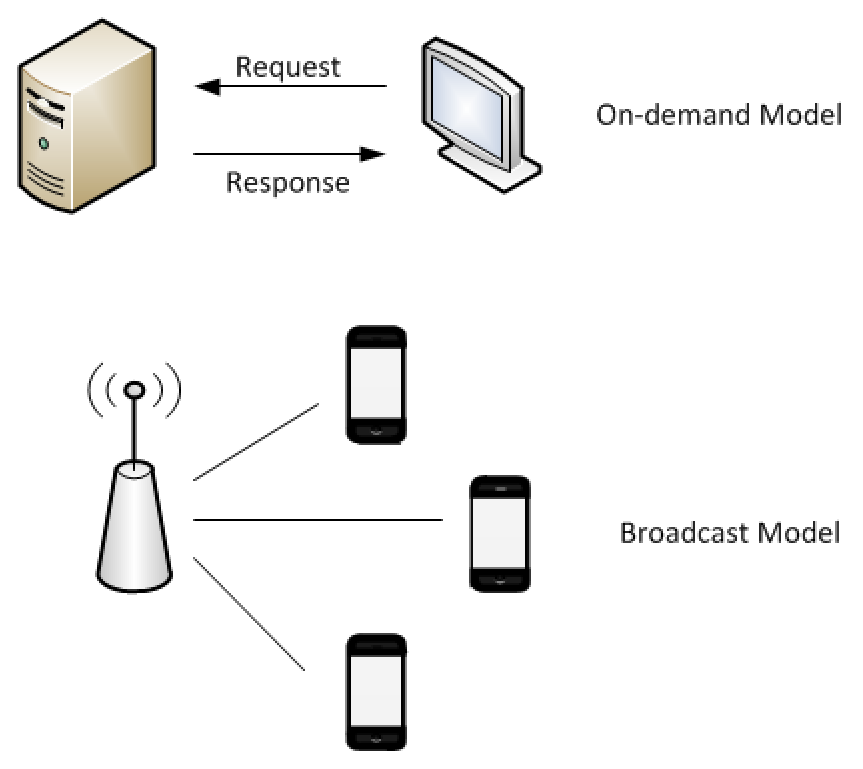
\includegraphics[width=2.5in]{Figures/on_demand.eps}
\caption{\small On demand and broadcast
models.\label{fig:broadcast}}
\end{center}
\end{figure}

A complete dissemination of all the records in the data set from
the server is a broadcast \emph{cycle}. A cycle follows another
cycle (see Figure~\ref{fig:bcast_cycle}). In this paper, we
sometime interchange cycle and program to denote the content of
the broadcast channel.

An inherit challenge of the broadcast model is the forward only
data model and that there is no random access of the data set.
When a client misses a piece of data from the current cycle, the
client must wait until the next cycle. The reverberations of these
properties of broadcast environment are: (1) we cannot adopt
disk-based skyline computation algorithms designed for traditional
database systems that require random access, and (2) we must
design a self-explanatory broadcast program using data index.

Many previous studies have done on different broadcast
environment. Multi-channels broadcast for data dissemination (and
techniques of data allocation) has been previously studied
\cite{DBLP:conf/cikm/HsuLC01} \cite{DBLP:conf/cikm/YeeN03}
\cite{DBLP:conf/mobicom/HameedV97}. Adaptive broadcast systems
that allow limited uplink (client to server) communication has
been studied in \cite{16350}. In this paper, we assume the
following properties for our broadcast environment:
\begin{enumerate}
\item Channel is forward-only. \item Only one channel is utilized.
\item No uplink bandwidth from clients to server.
\end{enumerate}

%The broadcast program is broken down into packets and each packet
%contains data records and each data record
%contains a number of fields (or attributes) as shown in
%Figure \ref{fig:bcast_cycle}. The entire broadcast program is considered
%a cycle. A new cycle is broadcasted after the cycle. Though the
%channel only broadcast one kind of data that is
%interesting to the clients, we assume that the data is different from one broadcast
%cycle to the next due to data updates between cycles. The consequence
%of different in data is that we cannot
%assume a records will broadcast at the same time in the next cycle and
%that the index structure could be vastly
%different between cycles.

\begin{figure}[h]
\begin{center}
\includegraphics[width=3.5in]{Figures/bcast_cycle.eps}
\caption{\small Broadcast program cycle}
\label{fig:bcast_cycle}
\end{center}
\end{figure}

Power consumption is a major concern since in this environment,
clients are small mobile devices, such as cellular phones, powered
by a small battery; therefore, power is an scarce and valuable
resource for these devices for most cases. Even for non-mobile
clients energy conservation is a desirable attribute for a system.
Actively listening to the broadcast channel is expensive in terms
of power usage. Most mobile devices is able to turn off the radio
receiver when it is not actively sending or receiving data to
conserve power.

To reduce the power consumption, an index is used to make the
broadcast cycle self-descriptive. As depicted in
Figure~\ref{fig:index_node}, An index provides additional
information in a broadcast program to tell the clients the
approximate time when a data records will be broadcasted. A
broadcast index is analogous to an index in traditional database
management systems in which the indexes provide the location of
data records and facilitate fast lookup of records. With the index
information, the clients can turn off the radio receiver and
transmitter to conserve power and only tune into the channel when
the desire data is being broadcasted.

%Similarly, wireless
%index tells the time when records will be broadcasted. With the index
%information, the clients can turn off the radio receiver and
%transmitter to conserve power and only tune into the channel when the
%desire data is being broadcasted. An example index would be for data
%in the range of [0, 10) will be broadcasted in time $t_1$, and for
%data in the range of [10, 20) will be broadcasted at time $t_2$ and so on
%as illustrated in Figure~\ref{fig:index_node}.

\begin{figure}[h]

\centering
\subfigure[2-D MBR]{
\includegraphics[width=1.4in]{Figures/mbr_2d.eps}
\label{fig:mbr_2d}
}
\subfigure[3-D MBR]{
\includegraphics[width=1.8in]{Figures/mbr_3d.eps}
\label{fig:mbr_2d}
}
\subfigure[]{
\includegraphics[width=1.8in]{Figures/index_node_entry.eps}
\label{fig:index_node_entry}
}
\caption{\small Tree Index.\label{fig:index_node}}
\end{figure}

%In this research, we study the way to embed data index in our
%broadcast program to provide efficient skyline query from broadcast
%program on air, while keeping the broadcast program useful to other
%applications. Our index technique is not overly specific as the index
%technique presented in \cite{Ha:2009:EEP:1616994.1617050} so that the
%broadcast program can only efficiently support skyline. In our
%technique we use generic, common tree index to be our index structure.
%Tree indexes are known to be generic and have been studied to support
%many other applications, for example range queries and k-nearest-neighbor
%($k$NN) queries. Since useful skyline queries involve multiple
%attributes, we utilize spatial indexes, such as R-Tree and R+-Tree,
%as our index structure although the data does not necessary contain
%spatial data in the sense of geo-spatial data. The relevant attributes
%forms a conceptual space in the spatial index. The reason we use spatial
%index so that multiple attributes can be indexed as shown in
%Figure~\ref{fig:skyline}. Existing wireless broadcast index techniques
%will be discussed in section \ref{sec:wireless_bcast_index}.

Adding index to a broadcast cycle also adds space overhead to the
cycle and ultimately consume more broadcast bandwidth. Quantities
that measure the efficiency of a wireless broadcast program are
defined below, of which \emph{tuning time} and \emph{access
latency} are well-known metrics and has been studied in other
works preceeding this paper \cite{dsi} \cite{data_on_air}
\cite{DBLP:journals/tmc/KuZW08} \cite{signature_and_caching}. We
also define \emph{Index Percentage} as a novel meansurement of the
space overhead of the index structure.

\begin{definition}[Index Percentage]\label{def:index_percentage}
The ratio of the space allocated to index to the space of the
entire cycle measure in bytes. This quantity is defined as $\rho =
\frac{\iota}{\omega}$.
\end{definition}

\begin{definition}[Initial Index Probe]\label{def:index_probe}
The amount of time for a client to get to the first index segment.
There are many methods of initial index probe, such as probing
every $\delta$ amount of time. Another method is to tune into the
channel the entire time until the first index is retrieved;
nonetheless this quantity is not added to the tuning time. This
quantity is denoted by $\alpha$.
\end{definition}

\begin{definition}[Tuning time]\label{def:tuning_time}
The total amount of time the client actively listening to the
channel in order to retrieve desire data. This is measured in
terms of the space of the index and data segments. This quantity
is denoted by $\beta$.
\end{definition}

\begin{definition}[Access latency]\label{def:access_latency}
The amount of time from when the client makes the request to when
the client receives all the desired data. Similar to tuning time,
this is also measured in terms of the space of the index and data
segments. This quantity is denoted by $\gamma$.
\end{definition}

%Skyline definition is definition~\ref{def:skyline},
%definition~\ref{def:index_percentage},
%definition~\ref{def:index_probe}
%By definition, the tuning time is directly proportional to the required energy consumption by the clients.
%Unfortunately, these two quantities are trade-offs for a broadcast program. When we try to reduce tuning
%time by including index, we increase the length of the program therefore increase access latency. If we
%do not include any index information, the program would be the shortest, but the client would have to listen
%to the entire program to get the desired data.
